% Created by tikzDevice version 0.10.1 on 2018-02-21 13:04:05
% !TEX encoding = UTF-8 Unicode
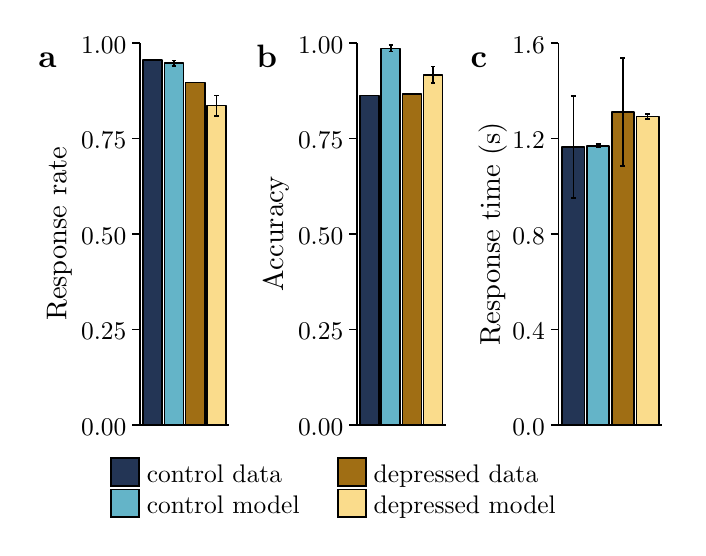
\begin{tikzpicture}[x=1pt,y=1pt]
\definecolor{fillColor}{RGB}{255,255,255}
\path[use as bounding box,fill=fillColor,fill opacity=0.00] (0,0) rectangle (234.88,180.67);
\begin{scope}
\path[clip] (  0.00, 28.91) rectangle ( 78.29,180.67);
\definecolor{drawColor}{RGB}{255,255,255}
\definecolor{fillColor}{RGB}{255,255,255}

\path[draw=drawColor,line width= 0.6pt,line join=round,line cap=round,fill=fillColor] (  0.00, 28.91) rectangle ( 78.29,180.67);
\end{scope}
\begin{scope}
\path[clip] ( 40.61, 37.16) rectangle ( 72.79,175.17);
\definecolor{fillColor}{RGB}{255,255,255}

\path[fill=fillColor] ( 40.61, 37.16) rectangle ( 72.79,175.17);
\definecolor{drawColor}{RGB}{0,0,0}
\definecolor{fillColor}{RGB}{35,53,85}

\path[draw=drawColor,line width= 0.6pt,line join=round,fill=fillColor] ( 41.76, 37.16) rectangle ( 48.65,169.08);
\definecolor{fillColor}{RGB}{100,180,200}

\path[draw=drawColor,line width= 0.6pt,line join=round,fill=fillColor] ( 49.42, 37.16) rectangle ( 56.32,167.82);
\definecolor{fillColor}{RGB}{160,110,20}

\path[draw=drawColor,line width= 0.6pt,line join=round,fill=fillColor] ( 57.08, 37.16) rectangle ( 63.98,160.91);
\definecolor{fillColor}{RGB}{250,220,140}

\path[draw=drawColor,line width= 0.6pt,line join=round,fill=fillColor] ( 64.75, 37.16) rectangle ( 71.64,152.49);

\path[draw=drawColor,line width= 0.6pt,line join=round] ( 52.10,168.80) --
	( 53.64,168.80);

\path[draw=drawColor,line width= 0.6pt,line join=round] ( 52.87,168.80) --
	( 52.87,166.84);

\path[draw=drawColor,line width= 0.6pt,line join=round] ( 52.10,166.84) --
	( 53.64,166.84);

\path[draw=drawColor,line width= 0.6pt,line join=round] ( 67.43,156.18) --
	( 68.96,156.18);

\path[draw=drawColor,line width= 0.6pt,line join=round] ( 68.19,156.18) --
	( 68.19,148.79);

\path[draw=drawColor,line width= 0.6pt,line join=round] ( 67.43,148.79) --
	( 68.96,148.79);
\end{scope}
\begin{scope}
\path[clip] (  0.00,  0.00) rectangle (234.88,180.67);
\definecolor{drawColor}{RGB}{0,0,0}

\path[draw=drawColor,line width= 0.6pt,line join=round] ( 40.61, 37.16) --
	( 40.61,175.17);
\end{scope}
\begin{scope}
\path[clip] (  0.00,  0.00) rectangle (234.88,180.67);
\definecolor{drawColor}{RGB}{0,0,0}

\node[text=drawColor,anchor=base east,inner sep=0pt, outer sep=0pt, scale=  0.92] at ( 35.66, 33.37) {0.00};

\node[text=drawColor,anchor=base east,inner sep=0pt, outer sep=0pt, scale=  0.92] at ( 35.66, 67.87) {0.25};

\node[text=drawColor,anchor=base east,inner sep=0pt, outer sep=0pt, scale=  0.92] at ( 35.66,102.38) {0.50};

\node[text=drawColor,anchor=base east,inner sep=0pt, outer sep=0pt, scale=  0.92] at ( 35.66,136.88) {0.75};

\node[text=drawColor,anchor=base east,inner sep=0pt, outer sep=0pt, scale=  0.92] at ( 35.66,171.39) {1.00};
\end{scope}
\begin{scope}
\path[clip] (  0.00,  0.00) rectangle (234.88,180.67);
\definecolor{drawColor}{RGB}{0,0,0}

\path[draw=drawColor,line width= 0.6pt,line join=round] ( 37.86, 37.16) --
	( 40.61, 37.16);

\path[draw=drawColor,line width= 0.6pt,line join=round] ( 37.86, 71.66) --
	( 40.61, 71.66);

\path[draw=drawColor,line width= 0.6pt,line join=round] ( 37.86,106.17) --
	( 40.61,106.17);

\path[draw=drawColor,line width= 0.6pt,line join=round] ( 37.86,140.67) --
	( 40.61,140.67);

\path[draw=drawColor,line width= 0.6pt,line join=round] ( 37.86,175.17) --
	( 40.61,175.17);
\end{scope}
\begin{scope}
\path[clip] (  0.00,  0.00) rectangle (234.88,180.67);
\definecolor{drawColor}{RGB}{0,0,0}

\path[draw=drawColor,line width= 0.6pt,line join=round] ( 40.61, 37.16) --
	( 72.79, 37.16);
\end{scope}
\begin{scope}
\path[clip] (  0.00,  0.00) rectangle (234.88,180.67);
\definecolor{drawColor}{RGB}{0,0,0}

\node[text=drawColor,rotate= 90.00,anchor=base,inner sep=0pt, outer sep=0pt, scale=  1.03] at ( 14.02,106.17) {Response rate};
\end{scope}
\begin{scope}
\path[clip] (  0.00,  0.00) rectangle (234.88,180.67);
\definecolor{drawColor}{RGB}{0,0,0}

\node[text=drawColor,anchor=base west,inner sep=0pt, outer sep=0pt, scale=  1.17] at (  3.83,166.18) {\bfseries a};
\end{scope}
\begin{scope}
\path[clip] ( 78.29, 28.91) rectangle (156.59,180.67);
\definecolor{drawColor}{RGB}{255,255,255}
\definecolor{fillColor}{RGB}{255,255,255}

\path[draw=drawColor,line width= 0.6pt,line join=round,line cap=round,fill=fillColor] ( 78.29, 28.91) rectangle (156.59,180.67);
\end{scope}
\begin{scope}
\path[clip] (118.99, 37.16) rectangle (151.09,175.17);
\definecolor{fillColor}{RGB}{255,255,255}

\path[fill=fillColor] (118.99, 37.16) rectangle (151.09,175.17);
\definecolor{drawColor}{RGB}{0,0,0}
\definecolor{fillColor}{RGB}{35,53,85}

\path[draw=drawColor,line width= 0.6pt,line join=round,fill=fillColor] (120.13, 37.16) rectangle (127.01,156.20);
\definecolor{fillColor}{RGB}{100,180,200}

\path[draw=drawColor,line width= 0.6pt,line join=round,fill=fillColor] (127.77, 37.16) rectangle (134.65,173.16);
\definecolor{fillColor}{RGB}{160,110,20}

\path[draw=drawColor,line width= 0.6pt,line join=round,fill=fillColor] (135.42, 37.16) rectangle (142.30,156.66);
\definecolor{fillColor}{RGB}{250,220,140}

\path[draw=drawColor,line width= 0.6pt,line join=round,fill=fillColor] (143.06, 37.16) rectangle (149.94,163.60);

\path[draw=drawColor,line width= 0.6pt,line join=round] (130.45,174.32) --
	(131.98,174.32);

\path[draw=drawColor,line width= 0.6pt,line join=round] (131.21,174.32) --
	(131.21,172.01);

\path[draw=drawColor,line width= 0.6pt,line join=round] (130.45,172.01) --
	(131.98,172.01);

\path[draw=drawColor,line width= 0.6pt,line join=round] (145.74,166.65) --
	(147.26,166.65);

\path[draw=drawColor,line width= 0.6pt,line join=round] (146.50,166.65) --
	(146.50,160.56);

\path[draw=drawColor,line width= 0.6pt,line join=round] (145.74,160.56) --
	(147.26,160.56);
\end{scope}
\begin{scope}
\path[clip] (  0.00,  0.00) rectangle (234.88,180.67);
\definecolor{drawColor}{RGB}{0,0,0}

\path[draw=drawColor,line width= 0.6pt,line join=round] (118.99, 37.16) --
	(118.99,175.17);
\end{scope}
\begin{scope}
\path[clip] (  0.00,  0.00) rectangle (234.88,180.67);
\definecolor{drawColor}{RGB}{0,0,0}

\node[text=drawColor,anchor=base east,inner sep=0pt, outer sep=0pt, scale=  0.92] at (114.04, 33.37) {0.00};

\node[text=drawColor,anchor=base east,inner sep=0pt, outer sep=0pt, scale=  0.92] at (114.04, 67.87) {0.25};

\node[text=drawColor,anchor=base east,inner sep=0pt, outer sep=0pt, scale=  0.92] at (114.04,102.38) {0.50};

\node[text=drawColor,anchor=base east,inner sep=0pt, outer sep=0pt, scale=  0.92] at (114.04,136.88) {0.75};

\node[text=drawColor,anchor=base east,inner sep=0pt, outer sep=0pt, scale=  0.92] at (114.04,171.39) {1.00};
\end{scope}
\begin{scope}
\path[clip] (  0.00,  0.00) rectangle (234.88,180.67);
\definecolor{drawColor}{RGB}{0,0,0}

\path[draw=drawColor,line width= 0.6pt,line join=round] (116.24, 37.16) --
	(118.99, 37.16);

\path[draw=drawColor,line width= 0.6pt,line join=round] (116.24, 71.66) --
	(118.99, 71.66);

\path[draw=drawColor,line width= 0.6pt,line join=round] (116.24,106.17) --
	(118.99,106.17);

\path[draw=drawColor,line width= 0.6pt,line join=round] (116.24,140.67) --
	(118.99,140.67);

\path[draw=drawColor,line width= 0.6pt,line join=round] (116.24,175.17) --
	(118.99,175.17);
\end{scope}
\begin{scope}
\path[clip] (  0.00,  0.00) rectangle (234.88,180.67);
\definecolor{drawColor}{RGB}{0,0,0}

\path[draw=drawColor,line width= 0.6pt,line join=round] (118.99, 37.16) --
	(151.09, 37.16);
\end{scope}
\begin{scope}
\path[clip] (  0.00,  0.00) rectangle (234.88,180.67);
\definecolor{drawColor}{RGB}{0,0,0}

\node[text=drawColor,rotate= 90.00,anchor=base,inner sep=0pt, outer sep=0pt, scale=  1.03] at ( 92.31,106.17) {Accuracy};
\end{scope}
\begin{scope}
\path[clip] (  0.00,  0.00) rectangle (234.88,180.67);
\definecolor{drawColor}{RGB}{0,0,0}

\node[text=drawColor,anchor=base west,inner sep=0pt, outer sep=0pt, scale=  1.17] at ( 82.67,166.18) {\bfseries b};
\end{scope}
\begin{scope}
\path[clip] (156.59, 28.91) rectangle (234.88,180.67);
\definecolor{drawColor}{RGB}{255,255,255}
\definecolor{fillColor}{RGB}{255,255,255}

\path[draw=drawColor,line width= 0.6pt,line join=round,line cap=round,fill=fillColor] (156.59, 28.91) rectangle (234.88,180.67);
\end{scope}
\begin{scope}
\path[clip] (191.81, 37.16) rectangle (229.38,175.17);
\definecolor{fillColor}{RGB}{255,255,255}

\path[fill=fillColor] (191.81, 37.16) rectangle (229.38,175.17);
\definecolor{drawColor}{RGB}{0,0,0}
\definecolor{fillColor}{RGB}{35,53,85}

\path[draw=drawColor,line width= 0.6pt,line join=round,fill=fillColor] (193.15, 37.16) rectangle (201.20,137.52);
\definecolor{fillColor}{RGB}{100,180,200}

\path[draw=drawColor,line width= 0.6pt,line join=round,fill=fillColor] (202.10, 37.16) rectangle (210.15,138.02);
\definecolor{fillColor}{RGB}{160,110,20}

\path[draw=drawColor,line width= 0.6pt,line join=round,fill=fillColor] (211.04, 37.16) rectangle (219.09,150.15);
\definecolor{fillColor}{RGB}{250,220,140}

\path[draw=drawColor,line width= 0.6pt,line join=round,fill=fillColor] (219.99, 37.16) rectangle (228.04,148.57);

\path[draw=drawColor,line width= 0.6pt,line join=round] (196.28,155.94) --
	(198.07,155.94);

\path[draw=drawColor,line width= 0.6pt,line join=round] (197.18,155.94) --
	(197.18,119.09);

\path[draw=drawColor,line width= 0.6pt,line join=round] (196.28,119.09) --
	(198.07,119.09);

\path[draw=drawColor,line width= 0.6pt,line join=round] (205.23,138.54) --
	(207.02,138.54);

\path[draw=drawColor,line width= 0.6pt,line join=round] (206.12,138.54) --
	(206.12,137.51);

\path[draw=drawColor,line width= 0.6pt,line join=round] (205.23,137.51) --
	(207.02,137.51);

\path[draw=drawColor,line width= 0.6pt,line join=round] (214.17,169.66) --
	(215.96,169.66);

\path[draw=drawColor,line width= 0.6pt,line join=round] (215.07,169.66) --
	(215.07,130.64);

\path[draw=drawColor,line width= 0.6pt,line join=round] (214.17,130.64) --
	(215.96,130.64);

\path[draw=drawColor,line width= 0.6pt,line join=round] (223.12,149.41) --
	(224.91,149.41);

\path[draw=drawColor,line width= 0.6pt,line join=round] (224.01,149.41) --
	(224.01,147.73);

\path[draw=drawColor,line width= 0.6pt,line join=round] (223.12,147.73) --
	(224.91,147.73);
\end{scope}
\begin{scope}
\path[clip] (  0.00,  0.00) rectangle (234.88,180.67);
\definecolor{drawColor}{RGB}{0,0,0}

\path[draw=drawColor,line width= 0.6pt,line join=round] (191.81, 37.16) --
	(191.81,175.17);
\end{scope}
\begin{scope}
\path[clip] (  0.00,  0.00) rectangle (234.88,180.67);
\definecolor{drawColor}{RGB}{0,0,0}

\node[text=drawColor,anchor=base east,inner sep=0pt, outer sep=0pt, scale=  0.92] at (186.86, 33.37) {0.0};

\node[text=drawColor,anchor=base east,inner sep=0pt, outer sep=0pt, scale=  0.92] at (186.86, 67.87) {0.4};

\node[text=drawColor,anchor=base east,inner sep=0pt, outer sep=0pt, scale=  0.92] at (186.86,102.38) {0.8};

\node[text=drawColor,anchor=base east,inner sep=0pt, outer sep=0pt, scale=  0.92] at (186.86,136.88) {1.2};

\node[text=drawColor,anchor=base east,inner sep=0pt, outer sep=0pt, scale=  0.92] at (186.86,171.39) {1.6};
\end{scope}
\begin{scope}
\path[clip] (  0.00,  0.00) rectangle (234.88,180.67);
\definecolor{drawColor}{RGB}{0,0,0}

\path[draw=drawColor,line width= 0.6pt,line join=round] (189.06, 37.16) --
	(191.81, 37.16);

\path[draw=drawColor,line width= 0.6pt,line join=round] (189.06, 71.66) --
	(191.81, 71.66);

\path[draw=drawColor,line width= 0.6pt,line join=round] (189.06,106.17) --
	(191.81,106.17);

\path[draw=drawColor,line width= 0.6pt,line join=round] (189.06,140.67) --
	(191.81,140.67);

\path[draw=drawColor,line width= 0.6pt,line join=round] (189.06,175.17) --
	(191.81,175.17);
\end{scope}
\begin{scope}
\path[clip] (  0.00,  0.00) rectangle (234.88,180.67);
\definecolor{drawColor}{RGB}{0,0,0}

\path[draw=drawColor,line width= 0.6pt,line join=round] (191.81, 37.16) --
	(229.38, 37.16);
\end{scope}
\begin{scope}
\path[clip] (  0.00,  0.00) rectangle (234.88,180.67);
\definecolor{drawColor}{RGB}{0,0,0}

\node[text=drawColor,rotate= 90.00,anchor=base,inner sep=0pt, outer sep=0pt, scale=  1.03] at (170.61,106.17) {Response time (s)};
\end{scope}
\begin{scope}
\path[clip] (  0.00,  0.00) rectangle (234.88,180.67);
\definecolor{drawColor}{RGB}{0,0,0}

\node[text=drawColor,anchor=base west,inner sep=0pt, outer sep=0pt, scale=  1.17] at (160.09,166.18) {\bfseries c};
\end{scope}
\begin{scope}
\path[clip] (  0.00,  0.00) rectangle (234.88,180.67);
\definecolor{fillColor}{RGB}{255,255,255}

\path[fill=fillColor] ( 19.47, -2.62) rectangle (215.41, 31.53);
\end{scope}
\begin{scope}
\path[clip] (  0.00,  0.00) rectangle (234.88,180.67);
\definecolor{drawColor}{RGB}{0,0,0}
\definecolor{fillColor}{RGB}{35,53,85}

\path[draw=drawColor,line width= 0.6pt,line cap=round,fill=fillColor] ( 30.21, 15.17) rectangle ( 40.17, 25.12);
\end{scope}
\begin{scope}
\path[clip] (  0.00,  0.00) rectangle (234.88,180.67);
\definecolor{drawColor}{RGB}{0,0,0}
\definecolor{fillColor}{RGB}{100,180,200}

\path[draw=drawColor,line width= 0.6pt,line cap=round,fill=fillColor] ( 30.21,  3.78) rectangle ( 40.17, 13.74);
\end{scope}
\begin{scope}
\path[clip] (  0.00,  0.00) rectangle (234.88,180.67);
\definecolor{drawColor}{RGB}{0,0,0}
\definecolor{fillColor}{RGB}{160,110,20}

\path[draw=drawColor,line width= 0.6pt,line cap=round,fill=fillColor] (112.19, 15.17) rectangle (122.15, 25.12);
\end{scope}
\begin{scope}
\path[clip] (  0.00,  0.00) rectangle (234.88,180.67);
\definecolor{drawColor}{RGB}{0,0,0}
\definecolor{fillColor}{RGB}{250,220,140}

\path[draw=drawColor,line width= 0.6pt,line cap=round,fill=fillColor] (112.19,  3.78) rectangle (122.15, 13.74);
\end{scope}
\begin{scope}
\path[clip] (  0.00,  0.00) rectangle (234.88,180.67);
\definecolor{drawColor}{RGB}{0,0,0}

\node[text=drawColor,anchor=base west,inner sep=0pt, outer sep=0pt, scale=  0.92] at ( 43.04, 16.36) {control data};
\end{scope}
\begin{scope}
\path[clip] (  0.00,  0.00) rectangle (234.88,180.67);
\definecolor{drawColor}{RGB}{0,0,0}

\node[text=drawColor,anchor=base west,inner sep=0pt, outer sep=0pt, scale=  0.92] at ( 43.04,  4.98) {control model};
\end{scope}
\begin{scope}
\path[clip] (  0.00,  0.00) rectangle (234.88,180.67);
\definecolor{drawColor}{RGB}{0,0,0}

\node[text=drawColor,anchor=base west,inner sep=0pt, outer sep=0pt, scale=  0.92] at (125.03, 16.36) {depressed data};
\end{scope}
\begin{scope}
\path[clip] (  0.00,  0.00) rectangle (234.88,180.67);
\definecolor{drawColor}{RGB}{0,0,0}

\node[text=drawColor,anchor=base west,inner sep=0pt, outer sep=0pt, scale=  0.92] at (125.03,  4.98) {depressed model};
\end{scope}
\end{tikzpicture}
